\documentclass{article}

\usepackage{graphicx}

\author{Dorian Arnold, Aurelien Bouteiller, George Bosilca,\\
 Kurt Feirrera, Thomas Herault, Yves Robert}
\title{Coordinated Checkpointing: Platform Perspective}

\begin{document}

\maketitle

Consider a platform with $p$ computing nodes. On this platform, at a given time job scheduler assigned $n$ applications that span on $S_{i, 1 \leq i \leq n}$ processors ($\sum_{i=1}^{n}S_i = p$). If each application uses coordinated checkpoint/restart and the same Daly formula for their checkpointing interval, is it possible to schedule all of them so that two applications never interfere?

Let $M$ be the average checkpoint size for a single node; let $b_{io}$ be the I/O bandwidth of the machine. For the sake of simplicity, consider first that there is no local I/O contention (the local link is not the bottleneck): Let $C(q)$ be the checkpoint duration of an application with $q$ nodes.

$$C(q) = q\times \frac{M}{b_{io}}$$

Let $\mu(q)$ be the MTBI of an application using $q$ nodes. By Daly, the optimal checkpoint interval of the application assuming no contention is $T_{opt}(q) = \sqrt{2C(q)\mu(q)}$. Assuming independent failures, $\mu(q) = \frac{\mu_{ind}}{q}$ (were $\mu_{ind}$ is the MTBF of a single node). Thus,

$$T_{opt}(q) = \sqrt{2\times q\times \frac{M}{b_{io}} \times \frac{\mu_{ind}}{q}} = \sqrt{2\frac{M}{b_{io}}\mu_{ind}} = T_{opt}$$

All applications checkpoint with the same interval, independent of their size (this is because the checkpoint duration is directly proportional to the number of nodes, while the chance of completing within the next time unit is inverse proportional to the same number of nodes).  To avoid contention, we thus must ensure that $\sum_{i = 1}^{n} C(S_i) \leq T_{opt}$, thus that

$$\begin{array}{rl}
\sum_{i = 1}^{n} S_i\times \frac{M}{b_{io}} & \leq \sqrt{2\frac{M}{b_{io}}\mu_{ind}}\\
p\frac{M}{b_{io}} & \leq \sqrt{2\frac{M}{b_{io}}\mu_{ind}}\\
b_{io} & \geq \frac{M\times p^2}{2\mu_{ind}}
\end{array}$$

Instantiating with $M = 8GB$, $p$ varying between 1,000 and 100,000, and $\mu_{ind}$ between 20 years and 80 years, we get Figure~\ref{fig:minio}. So... There is no problem? Indeed, if the platform can checkpoint a capacity application at the Daly optimal period, there is no problem. However, projected machines cannot do so for reasonable $\mu_{ind}$. Let's illustrate this in Figure~\ref{fig:projectedmachines}.

\begin{figure}[h!]
\begin{center}
  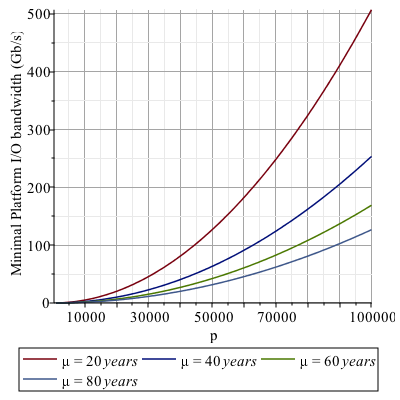
\includegraphics[width=.6\linewidth]{biomin.png}
\end{center}
\caption{Minimal platform I/O bandwidth requirement to allow independent checkpoint intervals\label{fig:minio}}
\end{figure}

\end{document}